\documentclass{article}
\usepackage[utf8]{inputenc}

\usepackage{graphicx}
\usepackage[spanish, es-tabla]{babel}
\usepackage{fullpage}
\usepackage{hyperref}
\usepackage{breakurl}
\usepackage{booktabs}
\usepackage{amsmath} 

\title{Resultados finales}
\author{Ionatan Perez}
\date{October 2016}

\begin{document}

\maketitle

\section{Planteo del experimento}


El objetivo general de la tesis es identificar y estudiar que variable influyen en el reconocimiento de patrones geometricos en la representacion sonora de las mismas mediante una codificacion tipo vOICe. En trabajos preliminares observamos que dicha capacidad depende drasticamente de la orientacion de los segmentos que componen las figuras en relacion a los ejes horizontales y verticales. Por ello las mediciones que realizamos a continuacion se centraron en observar dicha capacidad en figuras cuyos segmentos estuvieran orientados lejos de los ejes. 

El experimento realizado consistió en medir el nivel de umbral de deteccion de "paralalelismo" / "no paralelismo" y de "angulo recto" / "angulo no recto" en diferentes orientaciones, antes y despues de un proceso de entrenamiento. Para eso se diseñaron ocho orientaciones (cuatro de angulos y cuatro de paralelas).

Cada orientacion esta conformado por un conjunto de estimulos diferentes donde se generan variaciones en la medida que llamaremos señal o intensidad de señal y a su vez se genera variantes para cada intensidad de señal. En el caso de paralelismo la intensidad de señal es cuanto difiere (hacia ambos lados) el angulo formado por los segmentos del caso 0, es decir dos segmentos separados pero paralelos. En el caso de los angulos se genera un angulo formado por dos lados, uno que se mantiene fijo en la direccion dada por la orientacion y otro que varia formando angulos que difieren del angulo recto en la cantidad que llamamos señal. A su vez todos estos estimulos se rotan (en conjunto, ambos segmentos) levemente (bastante menos que la diferencia entre orientacion y orientacion) de manera de que para cada intensidad de señal haya multiples estimulos posibles. A los estimulos de señal 0 (segmentos paralelos o angulos rectos), tambien los denominamos estimulos neutros o sin señal. Todas las figuras estan centradas en el lienzo.

Cada experimento o nivel consiste en escuchar el sonido correspondiente a una serie de estimulos y responder si se trata de un estimulo neutro o con señal. Mediante un algoritmo tipo escalera se elijen dinamicamente los estimulos a mostrar de manera que la dificultad de la tarea aumente o disminuya en funcion de los aciertos o errores cometidos. El objetivo de cada nivel es determinar cual es el nivel de dificulad en el cual el usuario tiene la capacidad (estadistica) de reconocer correctamente una proporcion dada de los estimulos. En otras palabras, detectar el umbral de señal en el cual el usuario pasa de distinguir la mayor parte de los estimulos a no hacerlo. 

Los niveles diseñados pueden cumplir dos funciones diferentes, ser un nivel de evaluacion de la capacidad del sujeto (niveles tipo test) o ser un nivel diseñado para entrenar al sujeto (nivel entrenamiento). La principal diferencia es que en general en estos ultimos se porporciona feedback al usuario acerca de su respuesta y su longitud.

\section{Preguntas que se buscaron estudiar}

Al ajustar los parametros de la configuracion experimental se busco poder responder las siguientes preguntas:

\begin{itemize}
    \item ¿Cuan dificil le resulta a los usuarios reconocer las figuras en diferentes orientaciones previamente a cualquier entrenamiento?
    \item ¿Como afecta el entrenamiento la capacidad de reconocimiento de los patrones?
    \item ¿El entrenamiento realizado en una orientacion y geometria especifica, se transfiere a otras orientaciones y/o orientaciones?
\end{itemize}

Para responder estas preguntas decidimos realizar en los sujetos el siguiente protocolo:

\begin{enumerate}
    \item En una primera sesion, luego de un tutorial, realizamos a todos los sujetos una evaluacion (nivel tipo test) en ocho configuraciones de orientacion-categoria diferente. Evaluamos para las orientaciones 30º, 60º 120º y 150º en las categorias paralelismo y angulos. Llamamos a estas categorias P30, P60, P120, P150 y A30, A60, A120, A150 respectivamente. El orden mencionado de los niveles se mantuvo constante en todos los sujetos.
    
    La eleccion de orientaciones fue hecha de manera de tener una gran cantidad de simetrias. Como se puede observar en las figuras \ref{fig:simetriasAngulos} y \ref{fig:simetriasParalelismo}, las orientaciones 30 y 150 y 60 y 150 son simetricas respecto a la vertical en ambas categorias. Las paralelas tambien respetan esta simetria respecto a la horizontal, mientras que los angulos respetan simetria (asumiendo el caso de estimulos con angulos cercanos al recto) respecto a la horizontal entre 30 y 60 y 120 y 150 respectivamente. A su vez la simetria entre 30 y 60 o 120 y 150 en las paralelas esta dada por la reflexion a 45º. Por otra parte todos los estimulos de paralelismo tienen simetria de rotacion, mientras que los de angulos lo hacen de a pares (30 y 60 y 120 y 150) porque se rompe la simetria completa al dejar un lado "fijo". Dado que los valores finales de umbral son grandes en comparacion con las fluctuaciones que se generan dentro de cada "lado fijo" no se puede asumir que esta simetria se restituye. 
    
    \begin{figure}
        \centering
        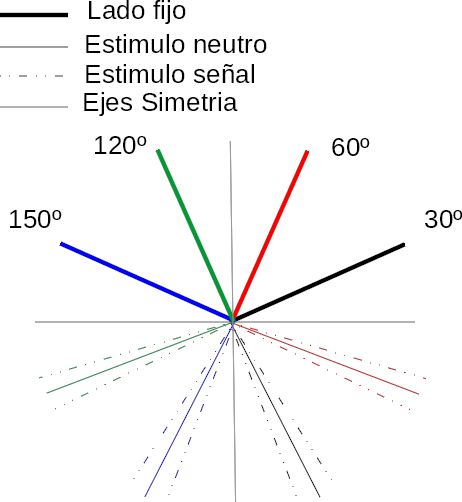
\includegraphics[width=0.3\textwidth]{Imagenes/SimetriasOrientacionAngulos.png}
        \caption{Orientaciones y simetrias para los estimulos de ángulos}
        \label{fig:simetriasAngulos}
    \end{figure}
    
        \begin{figure}
        \centering
        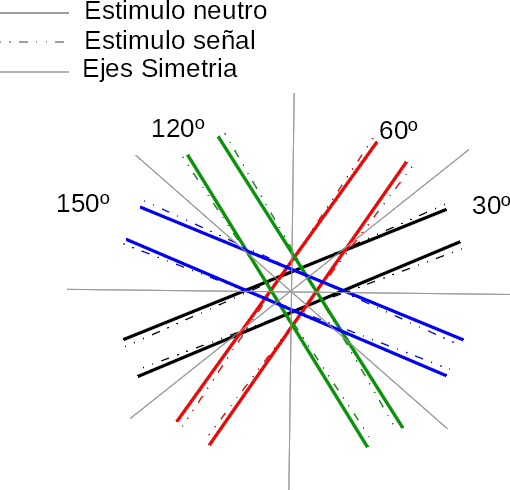
\includegraphics[width=0.3\textwidth]{Imagenes/SimetriasOrientacionParalelismo.png}
        \caption{Orientaciones y simetrias para los estimulos de paralelismo.}
        \label{fig:simetriasParalelismo}
    \end{figure}
    
    \item Entrenamos a algunos sujetos en la categoria P30 y a otros en la categoria A30. Para el entrenamiento se planeo cuatro sesiones (en dias diferentes entre si y diferentes al del test). En cada sesion se realizaron tres niveles, uno inicial con feedback, otro intermedio y mas corto sin feedback y uno final con feedback. Con este diseño se intento medir si al quitar el feedback se reducia la habilidad, si mejoraba igual o en menor medida. 
    
    \item Volvimos a realizar a todos los sujetos entrenados (y a otros tantos a modo de control) el mismo test que en la sesion inicial (sin el tutorial). 
    
\end{enumerate}

\section{Mediciones obtenidas}

    A partir del protocolo experimental diseñado se tomo datos para diez sujetos. La principal limitacion que llevo a un numero de sujetos tan bajo fue la longitud del experimento. Cada sujeto entrenado debio presentarse al laboratorio para tomas mediciones en seis oportunidades diferentes, por lo que, pese a ofrecer una retribucion economica no resulto facil conseguir sujetos que estuvieran dispuestos a participar en seis ocaciones y que tuviera compatibilidad horaria para que el experimento se dearrollara en un tiempo no extremadamente largo. 
    
    Con estas limitaciones entrenamos a dos sujetos en la categoria P30 y a dos en la categoria A30. Un quinto sujeto que no pudo completar el proceso de entrenamiento llego a hacer una sesion de entrenamiento en P30 y viendo los resultados preliminares le ofrecimos concluir el experimento en forma anticipada.
    
    Contando con estos 5 sujetos entrenados tambien medimos otros tantos sujetos a modo de control completando el conjunto de diez sujetos. 
    
    En las figuras \ref{fig:DatosTest} y \ref{fig:DatosEntrenamiento} se puede observar las medidas obtenidas para cada sujeto en cada uno de los niveles que realizo. El primer grafico muestra el desempeño para todos los sujetos, en la evaluacion previa y posterior al entrenamiento, y en el segundo grafico se muestra la evolución del sujeto a lo largo del entrenamiento para el caso de los sujetos que entrenaron.
    
    \begin{figure}
        \centering
        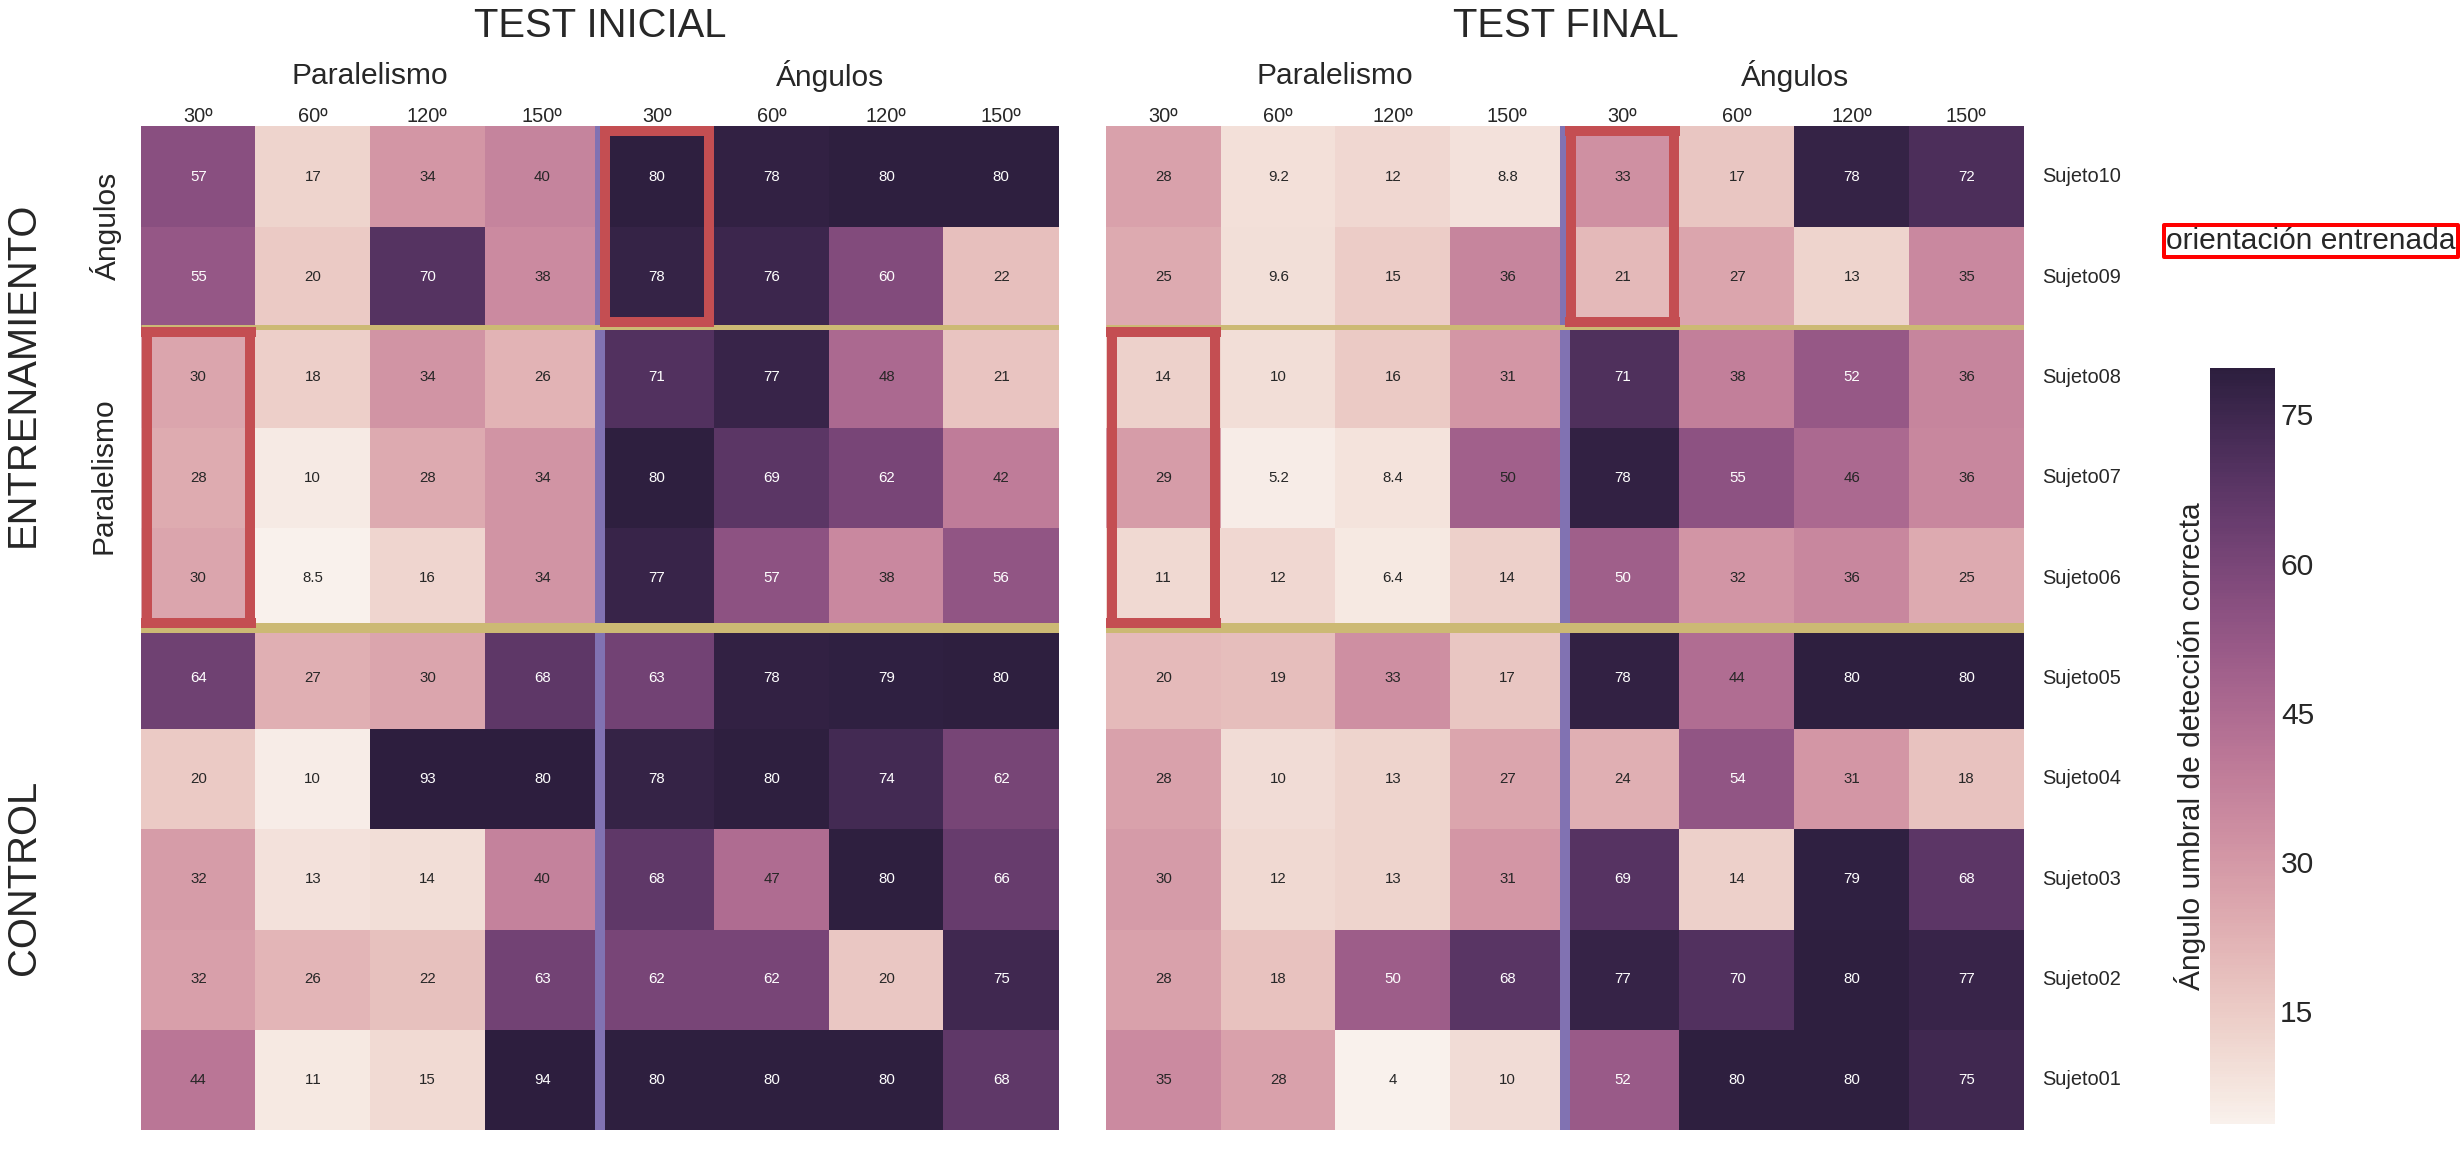
\includegraphics[width=\textwidth]{Imagenes/TransferenciaHeatmap.png}
        \caption{Mediciones para todos los sujetos comparando valores de umbral antes y despues del entrenamiento. Cada fila representa un sujeto.}
        \label{fig:DatosTest}
    \end{figure}
    
    \begin{figure}
        \centering
        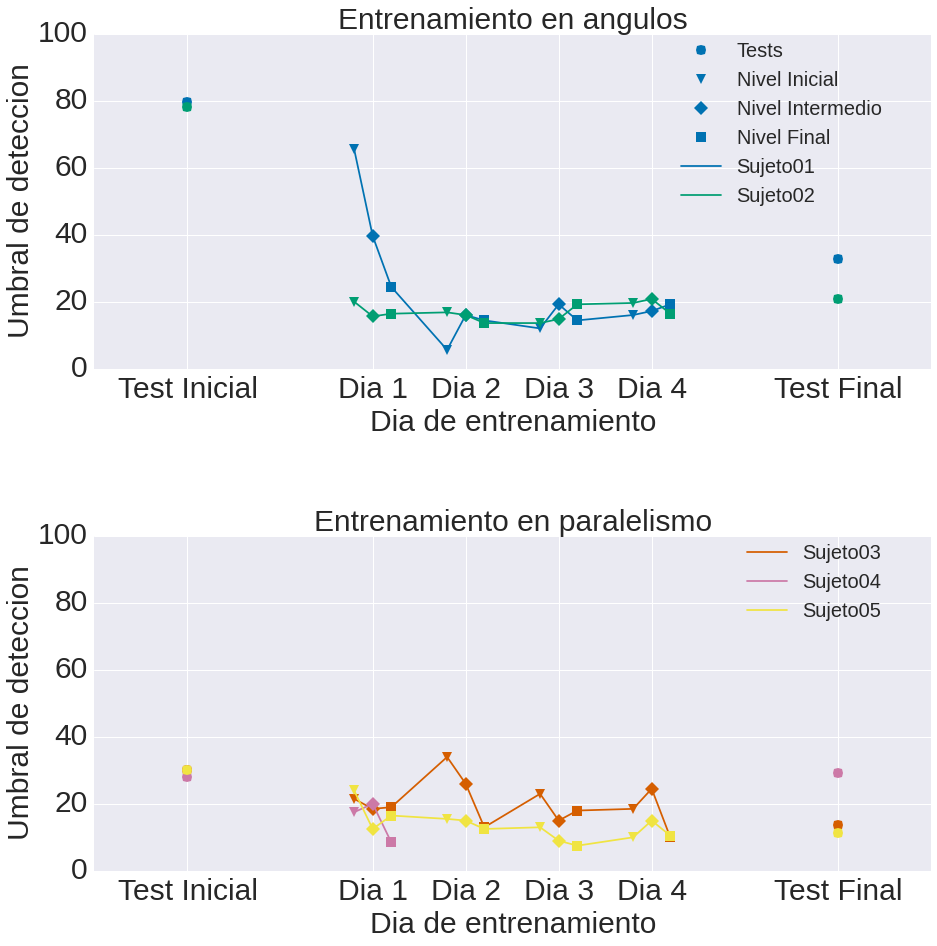
\includegraphics[width=\textwidth]{Imagenes/TransferenciaEntrenamientoNuevo.png}
        \caption{Evolucion de la capacidad de distinguir las categorias propuestas en funcion del entrenamiento. Cada color representa un usuario. En cada dias se realizan tres niveles diferentes, uno con feedback, uno sin, y otro con feedback igual al inicial.}
        \label{fig:DatosEntrenamiento}
    \end{figure}
    
\section{Resultados que se derivan de las mediciones}

El primer resultado que se puede observar a simple vista es que el entrenamiento satura muy rápido. En otras palabras que los sujetos alcanzan una performance alta al concluir el primer nivel de entrenamiento (que tiene feedback) y que ese nivel se mantiene mas o menos estable a lo largo de todo el proceso posterior de entrenamiento, excepto para un usuario que muestra una progresión durante el primer día. Tambien se puede observar que el proceso de mejora es mas notorio en el caso de los ángulos que en el caso del paralelismo. 

\subsection{Entrenamiento}

Para responder esta pregunta tomamos todas las medidas de umbral correspondientes a la categoria entrenada, separadas por sujeto. A esta secuencia de datos, los ajustamos con el siguiente modelo:


\begin{equation} \label{ec:RegresionEntrenamiento}
    %Y(i,t) = \alpha_i + \beta \cdot t + \gamma_{inicial} \Theta_{inicial} + \gamma_{final} \Theta_{final}
    Y(i,t) = \beta \cdot t + cte
\end{equation}

%donde i representa el sujeto, t el numero de nivel (o de mediciones ordenadas segun se realizaron), $\Theta$ un indicador de si el t corresponde al valor inicial o final de la serie (los tests), $\gamma$ el valor en que cambia el nivel medio de performance entre el test inicial o final y el entrenamiento (agrupado para todos los sujetos), $\alpha_{i}$ un factor fijo (parametro que ajusta sumando una constante agrupando por categoria) que mide la performance media por sujeto, y $\beta$ la pendiente de la performance durante el entrenamiento.

donde i representa el sujeto, t el numero de nivel (o de mediciones ordenadas segun se realizaron), $\beta$ la pendiente de la performance durante el entrenamiento, y cte una constante que brinda la libertad de ajustar la pendiente ingorando el valor medio de los datos. Recordemos que un $\beta$ negativo indica una mejora en la performance.

Ejemplificada para un caso de cuatro niveles de entrenamiento, y tres sujetos, quedaria un sistema de la forma de la ecuacion \ref{ec:MatrixExpandida}.

\begin{equation} \label{ec:MatrixExpandida}
    \bar {Y} = \bar{\delta} \cdot \bar{\bar{X}} \text{ con } \bar{\bar{X}} =
     \begin{pmatrix}
        %\beta & \alpha_1 & \alpha_2 & \alpha_3 & \gamma_{inicial} & \gamma_{final} \\
        0 & 1\\
        1 & 1\\
        2 & 1\\
        3 & 1\\
        0 & 1\\
        1 & 1\\
        2 & 1\\
        3 & 1\\
        0 & 1\\
        1 & 1\\
        2 & 1\\
        3 & 1\\
     \end{pmatrix} \text{ y $\bar{\delta}$ el conjunto de parametros para ajustar}
 \end{equation}

Analizando con este criterio todos los datos medidos (sin importar si entrenaron en ángulos o en paralelismo o si entrenaron todas las sesiones o menos) obtenemos los resultados que se observan en la tabla \ref{tabla:entrenamientoGlobal}.

\begin {table}

\begin{center}

\caption{Ejemplo de resultados obtenidos: caso de la regresión OLS para el conjunto de todas las mediciones durante entrenamiento, excluyendo la sesion outlier (dia 1, sujeto1}
\label{tabla:entrenamientoGlobal}

\vspace{0.3in}

\begin{tabular}{lclc}
\toprule
\textbf{Dep. Variable:}    &        y         & \textbf{  R-squared:         } &     0.026   \\
\textbf{Model:}            &       OLS        & \textbf{  Adj. R-squared:    } &     0.005   \\
\textbf{Method:}           &  Least Squares   & \textbf{  F-statistic:       } &     1.249   \\
\textbf{Date:}             & Fri, 04 Nov 2016 & \textbf{  Prob (F-statistic):} &    0.270    \\
\textbf{Time:}             &     15:28:40     & \textbf{  Log-Likelihood:    } &   -145.32   \\
\textbf{No. Observations:} &          48      & \textbf{  AIC:               } &     294.6   \\
\textbf{Df Residuals:}     &          46      & \textbf{  BIC:               } &     298.4   \\
\textbf{Df Model:}         &           1      & \textbf{                     } &             \\
\bottomrule
\end{tabular}

\begin{tabular}{lccccc}
               & \textbf{coef} & \textbf{std err} & \textbf{t} & \textbf{P$>|$t$|$} & \textbf{[95.0\% Conf. Int.]}  \\
\midrule
cte &      17.6615  &        1.386     &    12.746  &         0.000        &        14.872    20.451       \\
$\beta$    &      -0.2385  &        0.213     &    -1.117  &         0.270        &        -0.668     0.191       \\
\bottomrule
\end{tabular}

\begin{tabular}{lclc}
\textbf{Omnibus:}       &  8.165 & \textbf{  Durbin-Watson:     } &    1.476  \\
\textbf{Prob(Omnibus):} &  0.017 & \textbf{  Jarque-Bera (JB):  } &    8.482  \\
\textbf{Skew:}          &  0.639 & \textbf{  Prob(JB):          } &   0.0144  \\
\textbf{Kurtosis:}      &  4.616 & \textbf{  Cond. No.          } &     12.4  \\
\bottomrule
\end{tabular}

\end{center}

\end{table}

Como se puede observar en la figura \ref{tabla:betas}, ajustando la pendiente para todos los datos se puede observar que la pendiente da negativa y significativa. Sin embargo observando los datos en bruto de la figura \ref{fig:DatosEntrenamiento}, se ve que hay un sujeto que presenta una mejora notoria durante el primer dia. Si excluimos del ajuste el entrenamiento de ese sujeto, ese dia, la pendiente disminuye notoriamente y el ajuste indica que deja de ser significativamente distinta a cero. Este resultado se repite eliminando el primer dia para todos los sujetos o al sujeto en cuestion. Sin embargo en esta medicion estan analizados en conjunto quienes entrenan angulos y quienes entrenan paralelismo. Separando los datos en funcion del entrenamiento que realizaron, se puede ver que se incluya o no esa sesion de entrenamiento cada categoria por separado no muestra una mejora significativa a lo largo del entrenamiento. 

\begin {table}

\begin{center}

\caption{Resultados obtenidos para los ajustes de la pendiente y el efecto feedback considerando diferentes conjuntos de datos. Se observa que el unico caso donde se encontro un efecto significativo es en la mejora global del entrenamiento unificando todos los datos correspondientes las categorias de entrenamiento diferente y en la mejora intrasesion para el caso de paralelismo. \newline
* El usuario 1 presento un comportamiento marcadamente diferente durante el dia 1, por lo que se analizo los datos excluyendo estos datos \newline
** Datos excluyendo dia 1 del sujeto 1}
\label{tabla:betas}
\vspace{0.3in}

\begin{tabular}{lccccc}
            \textbf{Criterio utilizado} & \textbf{$\beta$} & $\alpha$ & \textbf{std err} & \textbf{t} & \textbf{P$>|$t$|$} \\%& \textbf{[95.0\% Conf. Int.]}\\
\midrule
\midrule
\textbf{Efecto del entrenamiento} &&&&&\\
\midrule
\textbf{Todos los datos medidos} & -0.8219 & &    0.346  &   -2.374  &    0.022     \\%&   -1.518    -0.126\\
Excluyendo usuario 1* &-0.1361 & &     0.244  &   -0.558   &    0.580     \\%&   -0.631     0.358 \\
Excluyendo dia 1 & -0.1292  & &   0.353 &    -0.365  &    0.717      \\%&  -0.848     0.589 \\
Excluyendo dia 1 usuario 1* & -0.2385 & &    0.213  &   -1.117  &    0.270       \\%& -0.668     0.191 \\
\textbf{Angulos (todos los datos)} & -1.1916 & &     0.646 &    -1.844 &     0.079     \\%&   -2.531     0.148\\
\textbf{Angulos sin dia 1 sujeto 1}* & 0.3126  & &   0.225  &    1.389  &    0.181      \\%&  -0.158     0.784 \\
\textbf{Paralelismo} & -0.5731    & &  0.322    & -1.779    &  0.087    \\%&    -1.237     0.090 \\
\midrule
\textbf{Efecto del entrenamiento en cada sesion} &&&&&\\
\midrule
\textbf{Angulos}** & 0.7143 & &    0.910     & 0.785     & 0.442      \\%&  -1.191     2.619\\
\textbf{Paralelismo} & -3.4167 & &     1.324  &   -2.580  &    \textbf{0.016}      \\%&  -6.144    -0.689 \\
\midrule
\textbf{Efecto de la ausencia de feedback} &&&&&\\
\midrule
\textbf{Angulos}** & & 1.5714    &  1.577    &  0.997    &  0.332    \\%&    -1.741     4.884\\
\textbf{Paralelismo}& & 1.0278   &   2.332   &   0.441   &   0.663   \\%&     -3.785     5.841\\
\bottomrule
\end{tabular}

\end{center}

\end{table}

Otra pregunta que se penso a la hora de diseñar el experimento fue evaluar la evolucion de la performance para cada sujeto, dentro del entrenamiento que se realiza en cada dia (sesion). El orden diario de entrenamiento fue un nivel con feedback, uno sin feedback y otro final igual al inicial. Las hipotesis a testear era dos, primero observar si habia un efecto olvido entre sesion y sesion que hiciera que la pendiente de performance dentro de cada sesion fuese mayor a la global del proceso de aprendizaje. La segunda hipotesis era observar si la inclusion de un nivel sin feedback producia un empeoramiento en el umbral medido, es decir si en la mejora medida se podia distinguir de una mejora debida exclusivamente al feedback, pero que no estuviera relacionada al proceso acumulado de aprendizaje. 

Para evaluar la primera de estas hipotesis se puede utilizar un modelo muy similar al de la ecuacion \ref{ec:RegresionEntrenamiento} pero haciendo que la variable t tome los valores 1, 2 y 3 y que el indice i represente no al usuario sino a cada sesion. El resultado obtenido se puede observar en la tabla \ref{tabla:betas} donde se ve que para el caso del entrenamiento en angulos no hay una pendiente significativa mientras que para el caso de paralelismo si. Como era de esperar la pendiente dio mucho mayor que la tendencia global, y esto se explica como un efecto serrucho donde entre sesion y sesion se pierde parte de la habilidad adquirida. 

Para evaluar la segunda pregunta, en el caso del entrenamiento en angulos podriamos realizar un test estadistico tipo T (luego de un Anova) entre los entrenamientos con feedback y los sin, ya que no parece haber una acumulacion de efecto debido al entrenamiento, sin embargo para el paralelismo esta hipotesis no se cumple. Un test que aplica a ambos casos es realizar un ajuste muy similar al hecho pero sumando un factor fijo en todas las mediciones intermedias, es decir un parametro que indique cuanto se le debe sumar al valor medio de las mediciones sin feedback para que de el valor esperado este sobre la recta que ajusta todos los datos. El importante notar que debido a la simetria del problema (sets de tres datos equiespaciados) sumar una constante a los valores intermedios no afecta el calculo de la pendiente. El modelo a ajustar es una leve variacion del anterior donde la matriz utilizada es la que se observa en la ecuacion \ref{ec:MatrizIntermedio}

\begin{equation} \label{ec:MatrizIntermedio}
    \bar {Y} = \bar{\delta} \cdot \bar{\bar{X}} \text{ con } \bar{\bar{X}} =
     \begin{pmatrix}
        0 & 0 & 1\\
        1 & 1 & 1\\
        2 & 0 & 1\\
        0 & 0 & 1\\
        1 & 1 & 1\\
        2 & 0 & 1\\
        0 & 0 & 1\\
        1 & 1 & 1\\
        2 & 0 & 1\\
        0 & 0 & 1\\
        1 & 1 & 1\\
        2 & 0 & 1\\
     \end{pmatrix} \text{ y $\bar{\delta}$ el conjunto de parametros para ajustar}
 \end{equation}
 
\subsection{Aprendizaje y transferencia}


\end{document}
